Были протестированы различные конфигурации группировки (аналог ''молнии'' и ''OneWeb''). Низкоорбитальные группировки обеспечивают хорошее покрытие и низкую задержку, однако поддержка актуального графа является сложной задачей.

\begin{figure}[H]
    \centering
    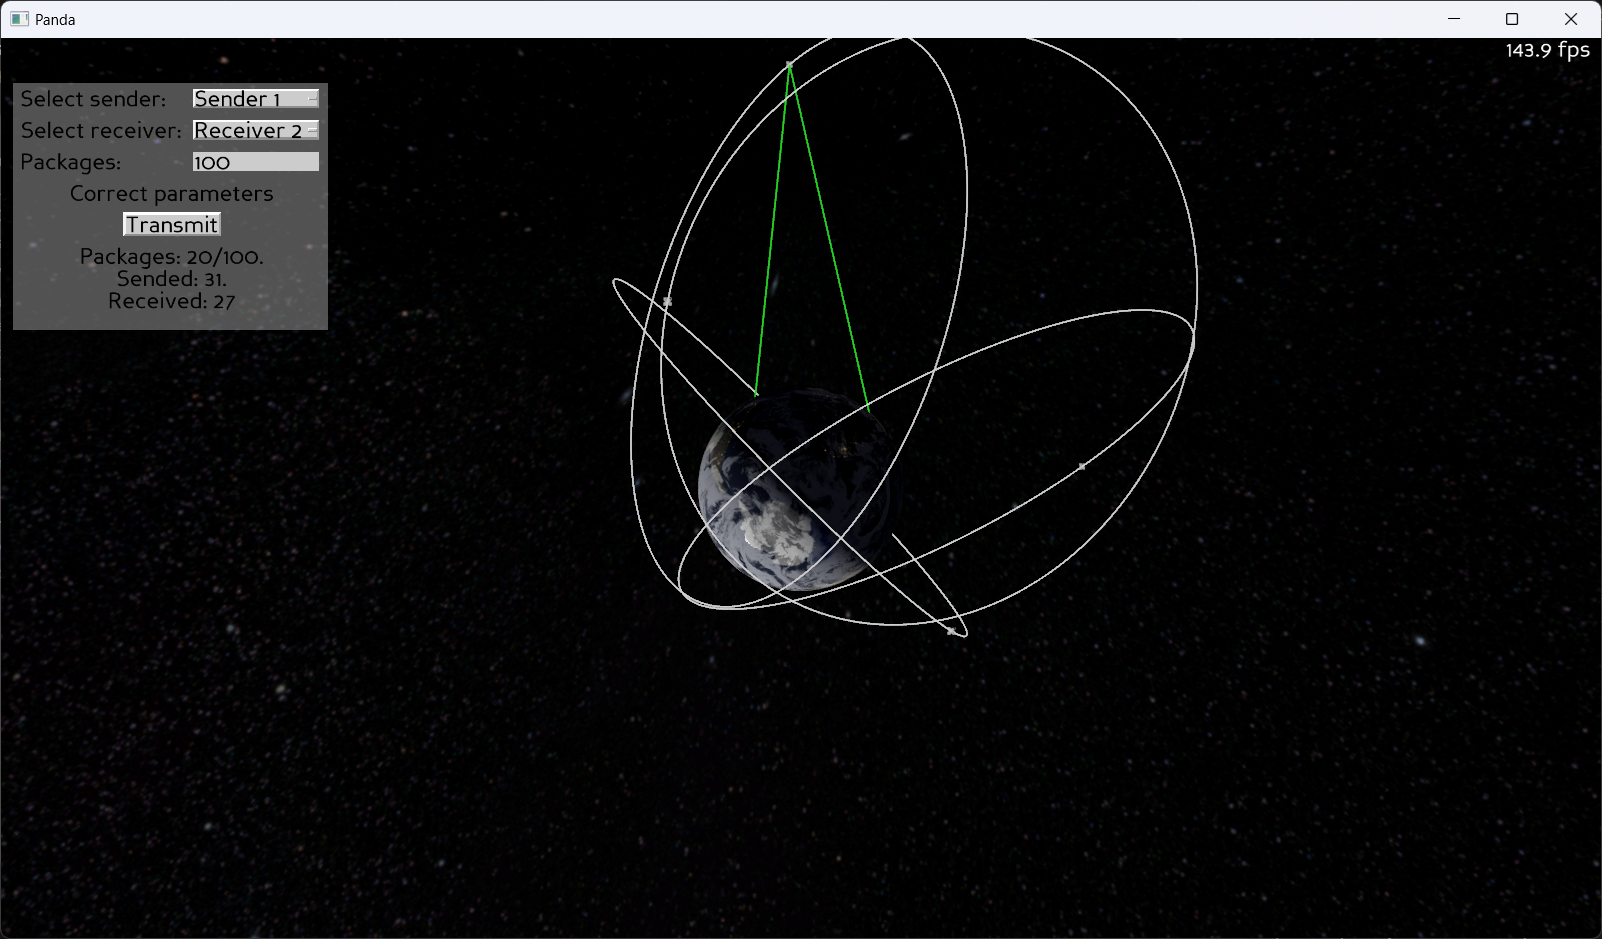
\includegraphics[width=0.9\linewidth]{image_1.png}
    \caption{Пример работы для аналога конфигурации ''молния''}
    \label{fig:image_1}
\end{figure}

\begin{figure}[H]
    \centering
    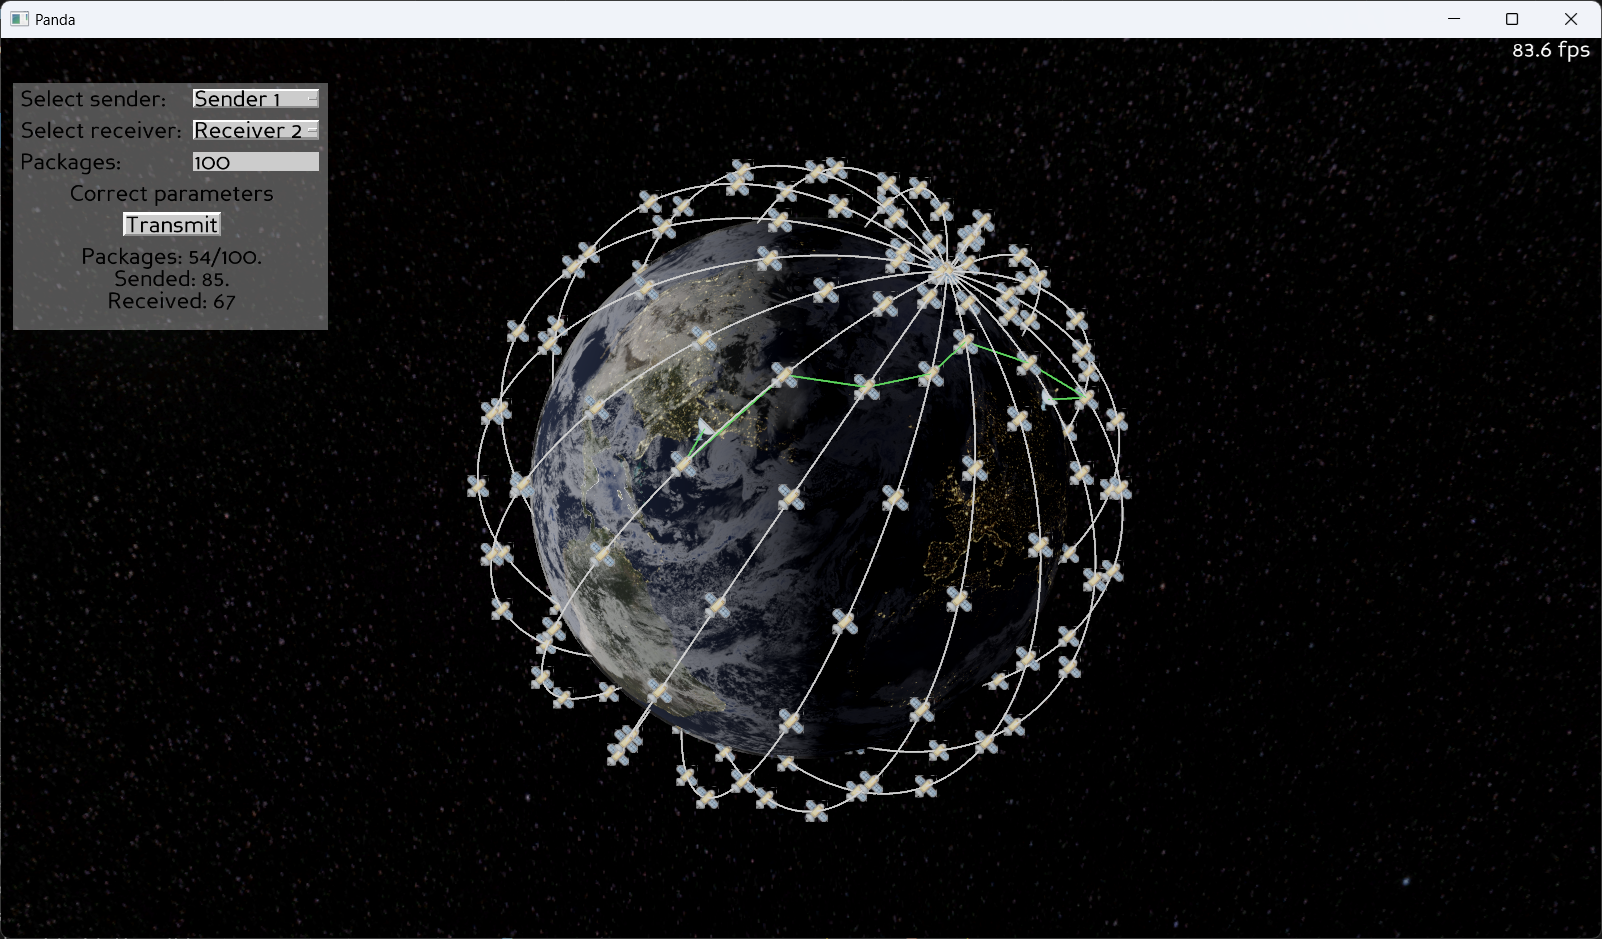
\includegraphics[width=0.9\linewidth]{image_2.png}
    \caption{Пример работы для аналога конфигурации ''OneWeb''}
    \label{fig:image_2}
\end{figure}